\documentclass[journal]{IEEEtran} % use the `journal` option for ITherm conference style
\IEEEoverridecommandlockouts
% The preceding line is only needed to identify funding in the first footnote. If that is unneeded, please comment it out.
\usepackage{hyperref}
\usepackage{cite}
\usepackage{amsmath,amssymb,amsfonts}
\usepackage{algorithmic}
\usepackage{graphicx}
\usepackage{textcomp}
\usepackage{xcolor}
\def\BibTeX{{\rm B\kern-.05em{\sc i\kern-.025em b}\kern-.08em
    T\kern-.1667em\lower.7ex\hbox{E}\kern-.125emX}}
\begin{document}

\title{Predictive Models in Patient Care: Predicting the Length of Stay for patients in Intensive Care Unit diagnosed with Pneumonia\\}

\author{%%%% author names
    \IEEEauthorblockN{João Carvalho}% first author
    % duplicate the line above as many times as needed to list all authors
    \\%%%% author affiliations
    \IEEEauthorblockA{\textit{DETI, Universidade de Aveiro}}\\% first affiliation
    \IEEEauthorblockA{\textit{Fundamentos de Aprendizagem Automática}}\\% delete this line if not needed
    % duplicate the line above as many times as needed to list all affiliations
    %%%% corresponding author contact details
    \IEEEauthorblockA{Prof. Petia Georgieva}
}

\maketitle

\begin{abstract}
The goal of this project is to apply machine learning (ML) algorithms in order to solve a specific data science problem. In this case, the purpose is to use supervised techniques to predict the Length of Stay(LOS) of patients in Intensive Care Unit(ICU) diagnosed with pneumonia. LOS can be defined as the number of days that an in-patient will remain in hospital during a single admission event. The data was collected in the scope
of a broader project that results from a scientific partnership
between \hyperlink{https://ritain.io}{Ritain.io} and the Institute of Electronics and Informatics Engineering of Aveiro, \hyperlink{http://www.ieeta.pt/}{IEETA} at University of Aveiro. This is a regression problem and, based on that, four ML models were implemented and evaluated: a Deep Learning model, an Artificial neural network model, a Random Forest model and a Linear Regression model. The best result was obtained by the Random Forest, and Deep learning models, which present the best evaluation metrics(R2=0.826 and R2=0.803). This kind of predictive analysis is a great help to the hospital resource management and valuable for supporting decisions of hospital managers.
\end{abstract}

\begin{IEEEkeywords}
    machine learning, regression, healthcare, length of stay (LOS)
\end{IEEEkeywords}

\section{Introduction}
Machine learning (ML) is a type of artificial intelligence (AI) that allows software applications to become more accurate at predicting outcomes. ML algorithms use historical data as input to predict new output values[7].
ML is growing in importance due to increasingly enormous volumes and variety of data. There are a large number of use cases that ML can be applied to in order to cut costs, reduce risks, and improve overall quality of life[8].
One of the areas where the use of ML has been growing is healthcare. Using ML for healthcare can open up a world of possibilities in this field, for example: improving diagnosis, developing new treatments, reducing costs and it enables to frees up healthcare providers' time to focus on patient care rather than searching or entering information \cite{JAVAID202258}.\newline

The goal of this project is to apply suitable ML algorithms to solve a specific data science problem, in this particular case, the purpose is to use supervised techniques to predict the Length of Stay(LOS) of patients in Intensive Care Unit(ICU) diagnosed with pneumonia. LOS can be defined as the number of days that an in-patient will remain in hospital during a single admission event, that is, is a clinical metric that measures the length of time elapsed between a patient's hospital admission and discharge. This metric is a crucial factor for the effective planning and management of hospital resources, hospital costs and increase service efficiency, besides that, it enables patients and their families to estimate the cost of a stay in paid hospitalizations. The LOS can be affected by some important factors such as: patient’s characteristics, presenting complaint, complications and discharge planning, as well as treatment complexity \cite{Stone2022}.\newline
In this work, the LOS is a continuous variable and measured in days, therefore, it will be treated as a regression problem. Four ML models will be tested to predict the LOS: a Deep Learning model, an Artificial Neural Network model, a Random Forest model and a Linear Regression model. In the next section, the practical implementation of the solution will be presented and discussed, and after that, the results and the models comparison will be analysed.

\section{Implementation}

This section presents the most relevant aspects regarding the data under analysis as well as the methods and their implementation details in Python.

\subsection{Data description and downsampling}
The data under analysis contains information of a large number of real patients admissions in ICU diagnosed with pneumonia, in Portugal.
The data was collected in the scope of a broader project that results from a scientific partnership between \hyperlink{https://ritain.io}{Ritain.io} and the Institute of Electronics and Informatics Engineering of Aveiro, \hyperlink{http://www.ieeta.pt/}{IEETA} at University of Aveiro. The data is confidential under a signed agreement between the parts and it has been properly anonymised in order to make sure that both individuals and institutions were no longer identifiable, complying with the GDPR requirements on collecting, storing and managing personal data.

The original dataset contains a total of 15.355 examples (admissions) and 102 variables with information related to the admissions, including personal information of the patient, medical prescriptions, relevant health metrics and, most importantly, the LOS value. Two approaches were considered to reduce the dimension of the dataset, namely by choosing some variables with predictive LOS value supported by the literature and by downsampling (in the admissions).
By one hand, the selection of the relevant features was supported by a literature search targeting this specific problem. Through the reading of several articles, the most relevant LOS predictive variables were identified and, if either existing or having a similar surrogate variable in the dataset, the variable was selected and used in this analysis. The literature review indicated that the patient age was an important factor for LOS prediction, where higher age tends to increase LOS ([9], [10], [11]). Moreover, other factors such as, the disease severity scores ([12], \cite{DBLP:journals/corr/abs-2201-00005}), lung or respiratory disorders ([13], \cite{Zolbanin2022}), infectious complications \cite{DBLP:journals/corr/abs-2201-00005} and admission type or diagnosis related group \cite{DBLP:journals/corr/abs-2201-00005} had a high association with the LOS value. Therefore, this work considered the following 8 predictive variables:
\begin{itemize}
    \item "DoenteIdadeEmAnos" (age), 
    \item "ServicoId" (service type), 
    \item "TipoAdmissaoId" (admission type), 
    \item "APACHEScore" (disease severity score), \item "SAPSScore" (disease severity score), \item "NumeroDiasEntubacao" (Intubation days), 
    \item "NumeroDiasVentilacaoInvasiva" (IV days), 
    \item "NrPrescricoesAntibiotico" (number of AP), 
\end{itemize}
where IV stands for "invasive ventilation" and AP stands for "antibiotic prescriptions". 
After variable selection, the downsampling process was performed by considered 10\% of the original examples without missing data in the selected variables, chosen at random, resulting in a sample of 1.294 examples.

In the Fig.1 is the statistical description of the final variables. And in the Fig. 2 is the distribution of the LOS value in the entire dataset and in the sample by the probability density function.\newline

\begin{figure}[htp]
    \centering
    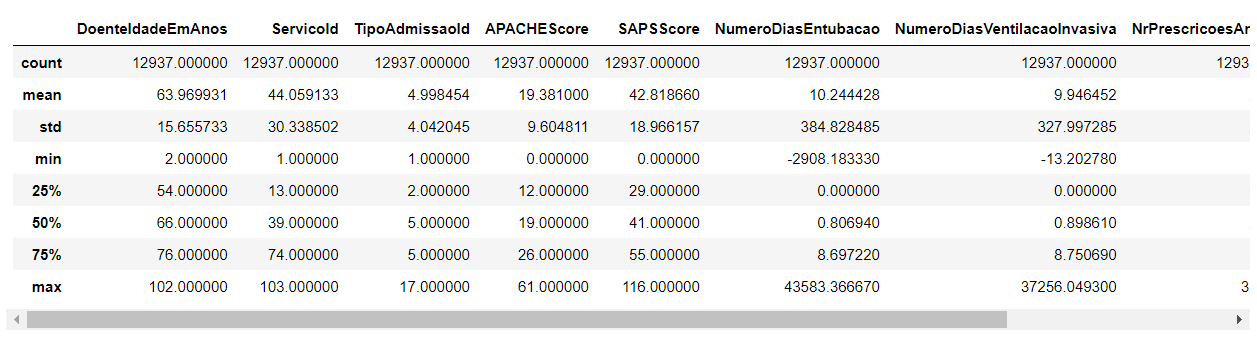
\includegraphics[width=8.5cm]{Project1-Report_FAA/dataset_desc.png}
    \caption{Dataset statistical description}
    \label{fig: adfgrg}
\end{figure}

\begin{figure}[htp]
    \centering
    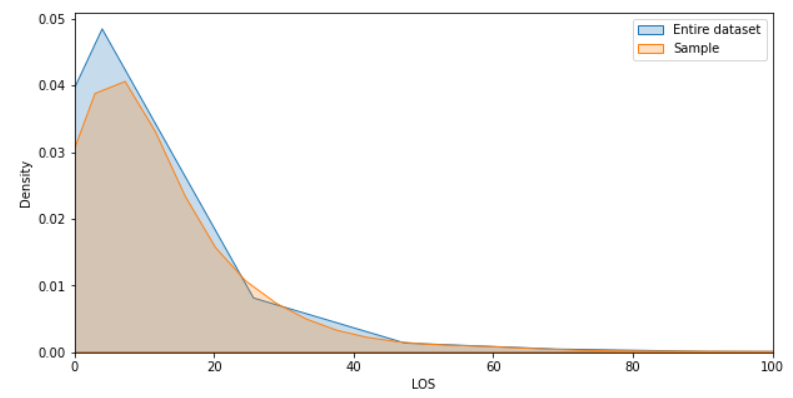
\includegraphics[width=9cm]{Project1-Report_FAA/density.png}
    \caption{The density plot of LOS}
    \label{fig:galaxy}
\end{figure}


%Another data preprocessing was the reduce of the total number of examples by a fraction of 10\%.
The Fig. 3 show the distibution of the variable LOS in the dataset with all examples and the Fig. 4 show the distibution of the variable LOS in the sample with 1.294. By analysing the two graphs we may see that the median LOS value of the complete dataset is very similar to the value of the sample, then, we may conclude that the group of examples extracted from the dataset is a good sample, in other words, is representative of the entire dataset.

\begin{figure}[htp]
    \centering
    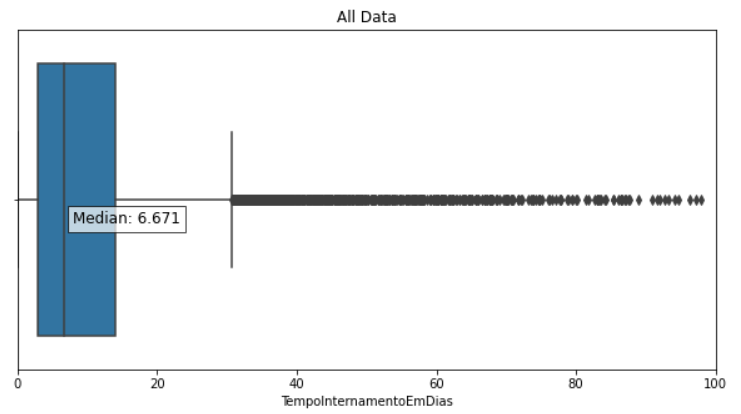
\includegraphics[width=8cm]{Project1-Report_FAA/box_los.png}
    \caption{LOS box plot in the entire dataset}
    \label{fig:galaxy}
\end{figure}


\begin{figure}[htp]
    \centering
    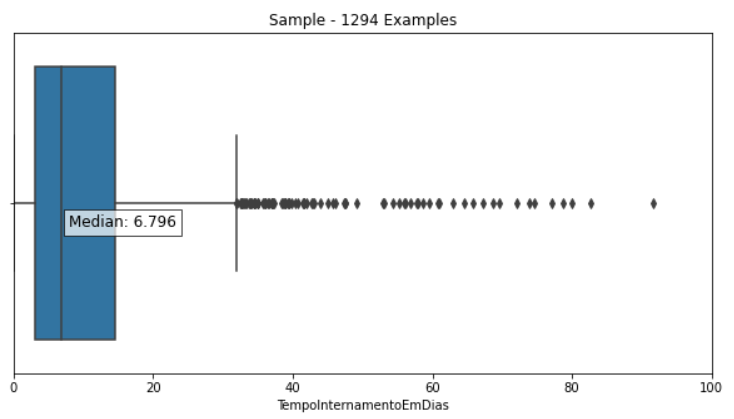
\includegraphics[width=8cm]{Project1-Report_FAA/box_los_sample.png}
    \caption{LOS box plot in the sample}
    \label{fig:galaxy}
\end{figure}

\subsection{Models}
This section includes a brief description of methods considered in this project, where the predictive models are presented in descending order complexity, namely deep learning (DL), artificial neural networks (ANN), random forest (RF) and linear regression (LR).
The \hyperlink{https://www.python.org/}{Python} implementation was based on the library \textit{Keras} (DL), the Multi-layer Perceptron regressor(MLPRegression) class from library \textit{Sklearn} (ANN), the \textit{RandomForestRegressor} class from library \textit{Sklearn} (RF) and the \textit{LinearRegression} class from \textit{Sklearn} (LR) as well as the class \textit{"Lasso"} from the library \textit{Sklearn} (LR by Lasso).\newline

\subsubsection{Deep Learning (DL)}
The development of DL models began with artificial neural networks, and it is essentially a neural network with three or more layers. A neural network with only one layer can still create approximations, but more hidden layers can help to improve and optimize for accuracy \cite{diagnostics11122242}. DL neural networks make use of bias, weights, and data inputs to try to imitate the workings of the human brain. These elements work together to accurately recognize, classify, and describe objects within the data.

The DL model constructed in this work, considered a network configuration equivalent to a DL model proposed in the literature for the same purpose of LOS prediction \cite{Zolbanin2022}. Namely, this model considered a network with a visible input layer with 59 neurons, five dense hidden layers (the first one with 128 and the others with 256 neurons each), and a single-neuron output layer. For each hidden layer, a Rectified Linear Units (ReLU) function as the layer’s activation (transfer) function was used. Since the network’s output has to be a real number(LOS), for the output layer was used a linear activation function .\newline 

\subsubsection{Artificial neural network (ANN)}
An ANN is a statistical model made up of a large number of densely, interconnected, adaptative and simple processing units - nodes(neurons) - working together to perform massively parallel computations for data processing[14]. ANNs are used in multivariate analysis to find both linear and non-linear relationships between data variables \cite{doi:10.4258/hir.2013.19.2.121}. In this approach, the following hyper-parameters were selected to be optimally tuned:
\begin{itemize}
  \item \textit{'hidden layer sizes'}: number of hidden layers and their number of neurons. Two hidden layers were tested, first trial was with 64 in the first one and 32 second one, second trial was with 32 in the first one and 12 second one, and finally with 12 and 6.
  \item \textit{'activation'}: activation function for the hidden layer. The activation functions used were 'relu','tanh'.
  \item \textit{'alpha'}: strength of the L2 regularization term. The alpha values used were 0.0001 and 0.05.
  \item \textit{'solver'}: the solver for weight optimization. The solver values used were ‘adam’ and ‘lbfgs’.
  \item \textit{'learning rate'}: learning rate schedule for weight updates. The learning rate values used were 'constant' and 'adaptive'.\newline
\end{itemize}

After trying all combinations, the optimal hyper-parameters were: hidden layer sizes=(32, 12),  activation='relu', alpha=0.0001, solver = 'adam' and learning rate = 'constant'.\newline

\subsubsection{Random Forest (RF)}
RF is a form of ensemble learning model made out of several decision trees. Ensemble learning models can integrate the outputs of various basic models to increase prediction accuracy \cite{diagnostics11122242}. There are three key hyper-parameters for RF algorithms that must be set prior to training. Node size, tree count, and sampled feature count are a few of them. From there, classification or regression issues can be resolved using the RF classifier. In this approach, the hyper-parameters selected were:
\begin{itemize}
  \item \textit{'n estimators'}: the number of trees in the forest. The values tested were 10, 50, 100, and 200.
  \item \textit{'max depth'}: the maximum depth of the tree. The values tested were 3, 10, 80, 90 and 110.\newline
\end{itemize}

After trying all combinations, the optimal hyper-parameters were: n estimators=100,  max depth=110.\newline

\subsubsection{Linear Regression (LR)}
LR is a type of analysis which involves one or more independent variables that may predict the value of the dependent variable through the calculation of the linear equation coefficients. This model fits a straight surface that minimizes the variance between predicted and actual output values [16]. LR models are relatively simple and provide an easy-to-understand mathematical formula that can generate predictions. In order to try to improve this method, the L1 prior as regularization technique(Lasso) was implemented with \textit{alpha} as hyper-parameter. The tested values for \textit{alpha} were 0.5, 0.05, 0.005, 0.0005, 1, 0.1, 0.01, 0.001 and 0.0001.\newline


After trying all possible values, the optimal model were Lasso with alpha = 0.1.

\subsection{Model training and validation}

Model validation refers to the process of evaluating a trained model with a testing data set. The main reason for using the testing dataset is to test the model's capacity to predict in the context of new data.

The validation of the models was based into two main approaches, namely Cross Validation (CV) and hyper-parameter selection (HPS). Fig. \ref{fig: jdfhla} presents a diagram representing the overall tasks involved in the validation of a model. Briefly, the dataset is divided into a set of training data (80\% of the data) and another set of test data (20\%). The training data is used to search for an optimal model, via HPS and cross-validation, which will have a final evaluation in the test data.

\begin{figure}[htp]
    \centering
    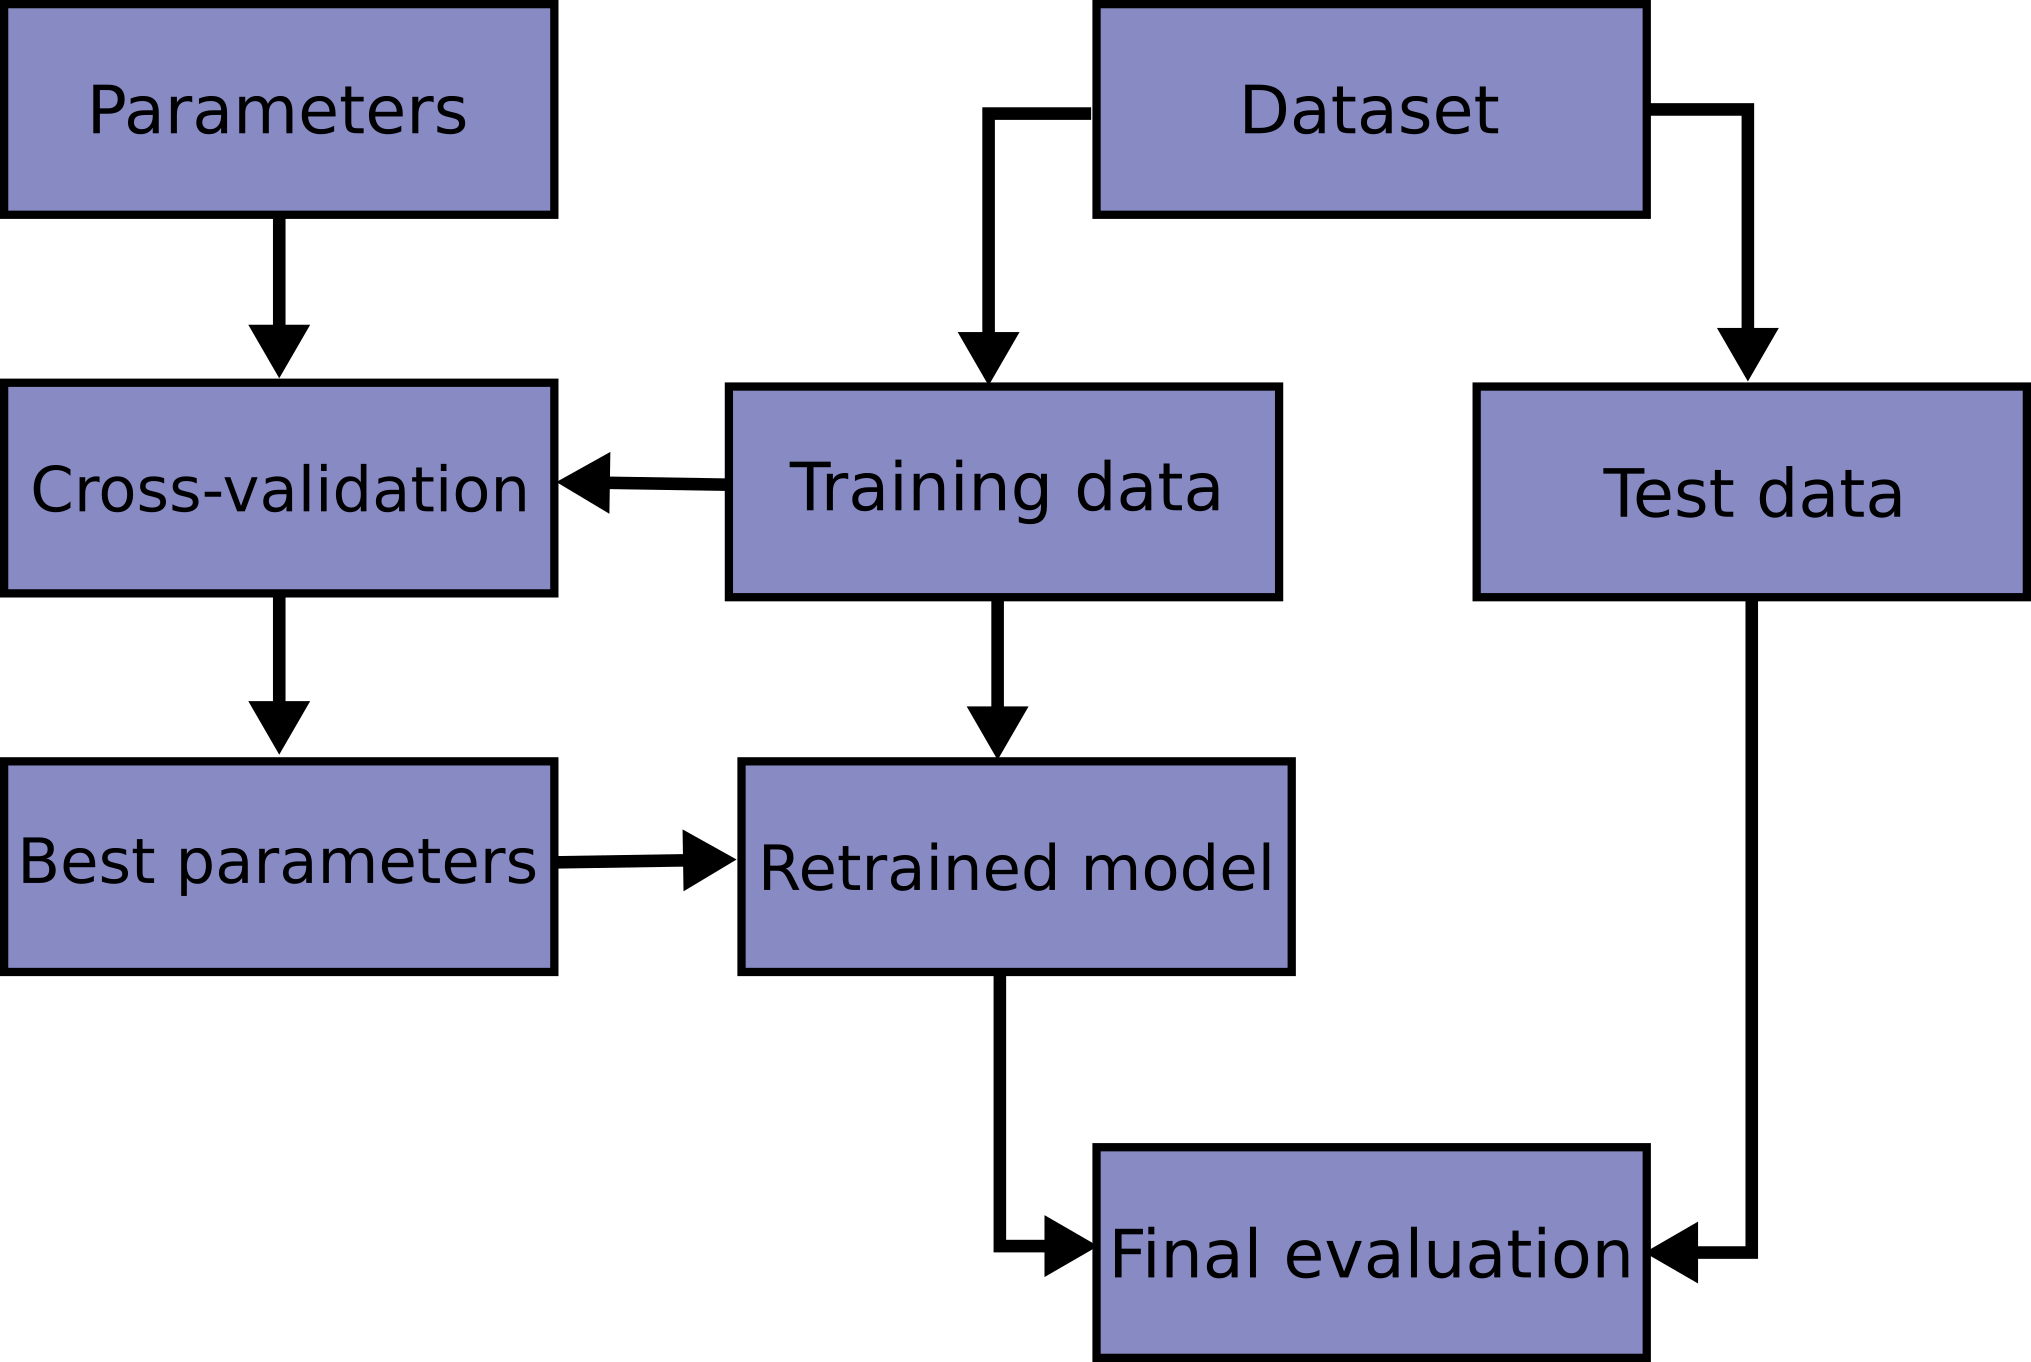
\includegraphics[width=8cm]{Project1-Report_FAA/grid_search_workflow.png}
    \caption{Diagram of models validation}
    \label{fig: jdfhla}
\end{figure}

In general, CV is a technique for assessing the performance of a machine learning model, helping in the comparison of different models and in the selection of a suitable model for the specific predictive modeling problem. This method consists of four main steps: (1) divide the dataset into training/test sets aiming the fitting and the validation of the model. In this work, CV was performed via $k$-Fold, by dividing the sample into $k=4$ groups of equal sizes, where the prediction function is learned using $k$-1 folds whereas the fold left out is used for test [17].

The HPS is the process of determining the combination of hyper-parameters or coefficients that maximizes the model performance. It operates by doing several trials within a single training procedure. Each trial is a complete execution of the CV algorithm with values for chosen hyper-parameters. This process once finished will give the set of hyper-parameter values that are best suited for the model to give optimal results [18]. The optimal hyper-parameters were chosen by minimisation of the Mean Square Error (MSE) over the model predictions.

\section{Results}
In this section the results will be analysed and discussed based on three metrics:
\begin{itemize}
  \item \textit{R2 Score(R2)}: Varies between 0 and 1. Is the proportion of the variance in the dependent variable that is predictable from the independent variable(s)[21]. Represents “1 - sum squared error(total variance not explained by model) / total variance” as demonstrated in the Fig. 6. 
  
  \begin{figure}[htp]
    \centering
    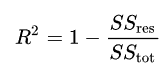
\includegraphics[width=4cm]{Project1-Report_FAA/r2_formula.png}
    \caption{R2 formula}
    \label{fig:galaxy}
\end{figure}
  
  \item \textit{Mean Absolute Percentage Error(MAPE)}: Represents the average of the absolute percentage errors of each entry in a dataset, showing, on average, how accurate the predicted values are in comparison with the real values[20].\newline
  
  \item \textit{Mean Squared Percentage Error(MSPE)}: Measures the amount of error in statistical models. It assesses the average squared difference between the observed and predicted values.[19]\newline
\end{itemize}

The graphics and tables below represent the results of running the models with the optimal hyper-parameters described in the section II.B.\newline

\begin{figure}[htp]
    \centering
    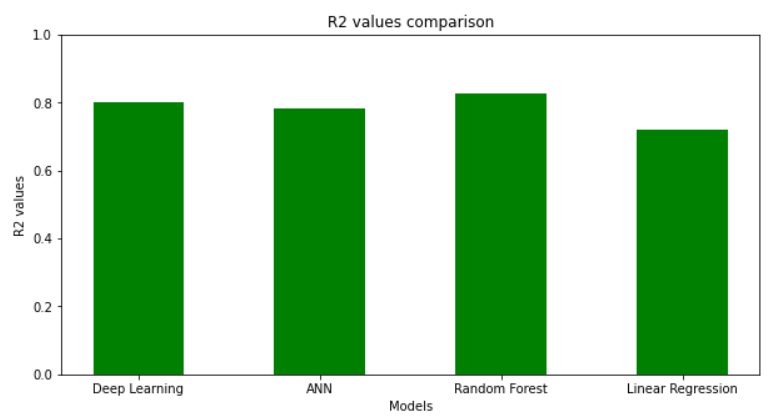
\includegraphics[width=8cm]{Project1-Report_FAA/r2.png}
    \caption{R2 value comparison between models}
    \label{fig:galaxy}
\end{figure}

\begin{figure}[htp]
    \centering
    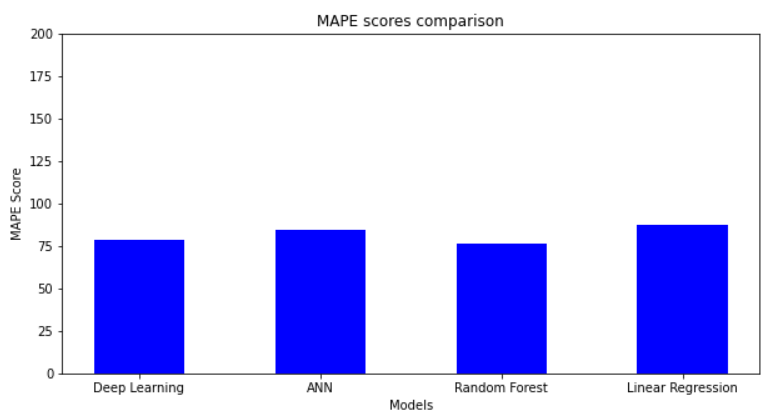
\includegraphics[width=8cm]{Project1-Report_FAA/mape.png}
    \caption{MAPE value comparison between models}
    \label{fig:galaxy}
\end{figure}

\begin{figure}[htp]
    \centering
    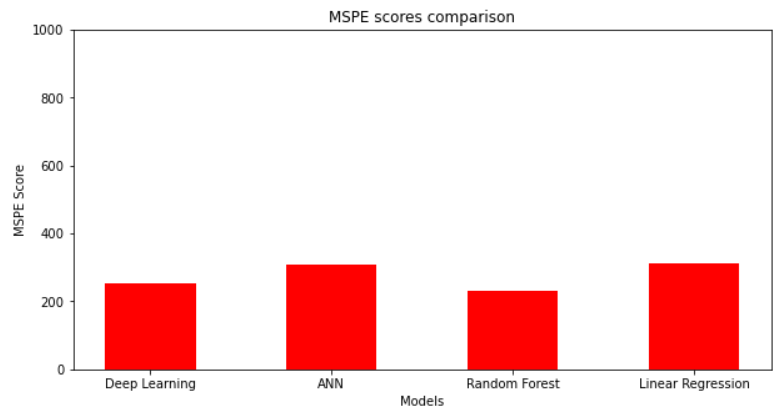
\includegraphics[width=8cm]{Project1-Report_FAA/mspe.png}
    \caption{MSPE value comparison between models}
    \label{fig:galaxy}
\end{figure}

\begin{figure}[htp]
    \centering
    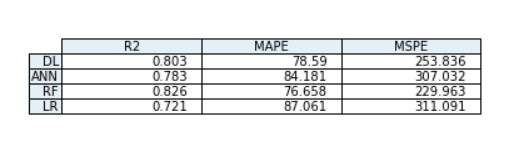
\includegraphics[width=6cm]{Project1-Report_FAA/metrics_table.png}
    \caption{Table with models and their metric values}
    \label{fig:galaxy}
\end{figure}

Observing the graphics and the table in particular, we may see that the results of the models are very similiar to each other. Apparently the DL and RF models had a little bit better behaviour than the LR and ANN in all metrics.

\section{Conclusion and Discussion}
The development of the ML field has created new exciting possibilities for the use of ML in several areas, including healthcare. In this work, a ML approach was
applied to estimate the LOS of patients in ICU diagnosed with pneumonia. Four models were implemented, validated and evaluated using three relevant metrics for regression problems. The RF and DL models got the best results with a R2 scores of 0.826 and 0.803 respectively. Comparing with the literature, it can be inferred that the results were reasonably good. The paper \cite{Zolbanin2022} obtained 0.655 and 0.613 for R2 values using ANN and the paper [5] got the R2 equals to 0.81 for the best model tested which was also a RF model.\newline
An important aspect to discuss is the performance/complexity trade-off of the models. Analyzing the results, it can be concluded that the most complex models, such as DL and ANN didn't bring performance improvement when working with small datasets.
For future work, it would be interesting to make a deeper analysis into the dataset variables in order to try to improve the model performance. Besides that, work with the entire dataset could give a different and relevant view of the models behavior.

% Use this is the final version
  %  unsrt produces numbered entries, sorted by order of citation
  %  plain produces numbered entries, sorted alphabetically
  %  other styles are possible (I recommend the harvard package)
  \bibliographystyle{unsrt}
  \bibliography{references}% replace by the name of name of your .bib file
  
\footnotesize{[7]https://www.techtarget.com/searchenterpriseai/definition/machine-learning-ML\newline
[8] https://www.microfocus.com/en-us/what-is/machine-learning\newline
[9] https://www.scitepress.org/Papers/2014/48922/48922.pdf\newline
[10] https://www.thespinejournalonline.com/article/S1529-9430(13)01617-3/fulltext\newline
[11] https://bmcanesthesiol.biomedcentral.com/articles/10.1186/1471-2253-7-8\newline
[12] https://pubmed.ncbi.nlm.nih.gov/12411659/\newline
[13] https://e-hir.org/journal/view.php?id=10.4258/hir.2013.19.2.121\newline
[14] https://www.sciencedirect.com/science/article/pii/S0933365707000528\newline
[16] https://www.ibm.com/topics/linear-regression\newline
[17] https://scikit-learn.org/stable/modules/cross\textunderscore validation.html\newline
[18] https://neptune.ai/blog/hyperparameter-tuning-in-python-complete-guide\newline
[19] https://statisticsbyjim.com/regression/mean-squared-error-mse/\newline
[20] https://www.indeed.com/career-advice/career-development/what-is-mape\newline
[21] https://www.bmc.com/blogs/mean-squared-error-r2-and-variance-in-regression-analysis/}
\end{document}
